\PassOptionsToPackage{xetex}{xcolor}
\PassOptionsToPackage{xetex}{graphicx}
\documentclass[a4paper,landscape,headrule,footrule,xetex]{foils}

%%
%%% macros for 2009 Semester 1 HG 803
%%%
\newcommand{\logo}{~}
\newcommand{\header}[3]{%
  \title{\vspace*{-2ex} \large HG3051  Corpus Linquistics
    \\[2ex] \Large  \emp{#2} \\ \emp{#3}}
  \author{\blu{Francis Bond}   \\ 
    \normalsize  \textbf{Division of Linguistics and Multilingual Studies}\\
    \normalsize  \url{http://www3.ntu.edu.sg/home/fcbond/}\\
    \normalsize  \texttt{bond@ieee.org}}
  \MyLogo{HG3051 (2018)}
  \renewcommand{\logo}{#2}
  \hypersetup{
    pdfinfo={
      Author={Francis Bond},
      Title={#1: #2},
      Subject={HG3051: Corpus Linguistics},
      Keywords={Corpus Linguistics},
      License={CC BY 4.0}
    }
  }
  \date{#1 \\ \url{https://github.com/bond-lab/Corpus-Linguistics}}
}

\usepackage{fontenc}
\usepackage{polyglossia}
\setmainlanguage{english}
\setmainfont{TeX Gyre Pagella}
%\setmainfont{Linux Libertine}
%\setmainfont{Charis SIL}
\newfontfamily{\ipafont}{Gentium}
\newcommand{\ipa}[1]{{\ipafont\selectfont #1}}
\usepackage{xeCJK}

\setCJKmainfont{Noto Sans CJK SC}
\setCJKsansfont{Noto Sans CJK SC}



\usepackage{xcolor}
\usepackage{graphicx}
\newcommand{\blu}[1]{\textcolor{blue}{#1}}
\newcommand{\grn}[1]{\textcolor{green}{#1}}
\newcommand{\hide}[1]{\textcolor{white}{#1}}
\newcommand{\emp}[1]{\textcolor{red}{#1}}
\newcommand{\txx}[1]{\textbf{\textcolor{blue}{#1}}}
\newcommand{\lex}[1]{\textbf{\mtcitestyle{#1}}}

\usepackage{pifont}
\renewcommand{\labelitemi}{\textcolor{violet}{\ding{227}}}
\renewcommand{\labelitemii}{\textcolor{purple}{\ding{226}}}

\newcommand{\subhead}[1]{\noindent\textbf{#1}\\[5mm]}

\newcommand{\Bad}{\emp{\raisebox{0.15ex}{\ensuremath{\mathbf{\otimes}}}}}
\newcommand{\bad}{*}

\newcommand{\com}[1]{\hfill \textnormal{(\emp{#1})}}%
\newcommand{\cxm}[1]{\hfill \textnormal{(\txx{#1})}}%
\newcommand{\cmm}[1]{\hfill \textnormal{(#1)}}%

\usepackage{relsize,xspace}
\newcommand{\into}{\ensuremath{\rightarrow}\xspace}
\newcommand{\ent}{\ensuremath{\Rightarrow}\xspace}
\newcommand{\nent}{\ensuremath{\not\Rightarrow}\xspace}
\newcommand{\tot}{\ensuremath{\leftrightarrow}\xspace}
\usepackage{url}
\newcommand{\lurl}[1]{\MyLogo{\url{#1}}}

\usepackage{mygb4e}
\let\eachwordone=\itshape
\newcommand{\lx}[1]{\textbf{\textit{#1}}}

%\usepackage{times}
%\usepackage{nttfoilhead}
\newcommand{\myslide}[1]{\foilhead[-25mm]{\raisebox{12mm}[0mm]{\emp{#1}}}\MyLogo{\logo}}
\newcommand{\myslider}[1]{\rotatefoilhead[-25mm]{\raisebox{12mm}[0mm]{\emp{#1}}}}
%\newcommand{\myslider}[1]{\rotatefoilhead{\raisebox{-8mm}{\emp{#1}}}}

\newcommand{\section}[1]{\myslide{}{\begin{center}\Huge \emp{#1}\end{center}}}



\usepackage[lyons,j,e,k]{mtg2e}
\renewcommand{\mtcitestyle}[1]{\textcolor{teal}{\textsl{#1}}}
%\renewcommand{\mtcitestyle}[1]{\textsl{#1}}
\newcommand{\chn}{\mtciteform}
\newcommand{\cmn}{\mtciteform}
\newcommand{\iz}[1]{\textup{\texttt{\textcolor{blue}{\textbf{#1}}}}}
\newcommand{\rel}[1]{\textsc{\color{blue}{#1}}}
\newcommand{\wn}[3]{\lex{#1}\ensuremath{_{#2:#3}}}
\newcommand{\con}[1]{\textsc{#1}}
\newcommand{\gm}{\textsc}
\usepackage[normalem]{ulem}
\newcommand{\ul}{\uline}
\newcommand{\ull}{\uuline}
\newcommand{\wl}{\uwave}
\newcommand{\vs}{\ensuremath{\Leftrightarrow}~}
\usepackage[hidelinks]{hyperref}
\hypersetup{
     colorlinks,
     linkcolor={blue!50!black},
     citecolor={red!50!black},
     urlcolor={blue!80!black}
}
%%%
%%% Bibliography
%%%
\usepackage{natbib}
%\usepackage{url}
\usepackage{bibentry}
%%% From Tim
\newcommand{\WMngram}[1][]{$n$-gram#1\xspace}
\newcommand{\infers}{$\rightarrow$\xspace}


\header{Lecture 2}{Markup and Annotation}{}

\usepackage{pst-node}
\newcommand{\sa}[2]{\rnode{c#1}{\iz{#2}}}%\nodebox{c#1}}



\begin{document}
\maketitle


\myslide{Overview}

\begin{itemize} 
\item Revision of Introduction
  \begin{itemize}
  \item What is Corpus Linguistics
  \end{itemize}
\item \blu{Mark-up}
\item \blu{Annotation}
\item \blu{Regular Expressions}
\item \textbf{Lab One}
\end{itemize}

%%%
%%% this changes each year, so keep separate
%%%
\include{schedule}

\section{Revision}


\myslide{What is a Corpus?}

\lx{corpus} (pl: \lx{corpora}):
\begin{itemize}
\item In linguistics and lexicography, a body of texts, utterances, or other
specimens considered more or less representative
of a language, and usually stored as an electronic
database. 
  \begin{itemize}
  \item machine-readable (i.e., computer-based)
  \item authentic (i.e., naturally occurring)
  \item sampled (bits of text taken from multiple sources)
  \item representative of a particular language or language variety.
  \end{itemize}
\item  Sinclair's (1996) definition:
  \begin{quote}
    A corpus is a collection of pieces of language that are selected and
    ordered according to explicit linguistic criteria in order to be used as a
    sample of the language.
\end{quote}
% \item Corpus linguistics is the study of language as expressed in samples
% (corpora) or ``real world'' text.
\end{itemize}


\myslide{Why Are Electronic Corpora Useful?}
\begin{itemize}
\item as a collection of examples for linguists
  \begin{itemize}
  \item intuition is unreliable
  \end{itemize}
\item as a data resource for lexicographers
  \begin{itemize}
  \item use natural data to exemplify usage
  \end{itemize}
\item as instruction material for language teachers and learners
\item as training material for natural language processing applications
  \begin{itemize}
  \item training of speech recognizers, parsers, MT
  \end{itemize}
\end{itemize}



\myslide{The British National Corpus (BNC)}
\begin{itemize}
\item 100 million words of written and spoken British English
\item Designed to represent a wide cross-section of British English from late 20th century: balanced and representative
\item POS tagging (2 million word sampler hand checked)
\end{itemize}
\begin{small}
  \begin{tabular}{l|lll}
    Written  & Domain  & Date & Medium \\ \hline
    (90\%)  & Imaginative (22\%) & 1960-74 (2\%) & Book (59\%) \\
    & Arts (8\%) & 1975-93 (89\%)  & Periodical (31\%)   \\
    & Social science (15\%)  & Unclassified (8\%)  & Misc. published (4\%) \\
    & Natural science (4\%) \ldots  & & Misc. un-pub (4\%)    \\  \hline
    Spoken  & Region  & Interaction type  & Context-governed \\ \hline
    (10\%)  &  South (46\%)  & Monologue (19\%)  & Informative (21\%) \\
    & Midlands (23\%)  & Dialogue (75\%)  & Business (21\%) \\
    & North (25\%)  \ldots & Unclassified (6\%)  & Institutional (22\%)  \ldots\\
  \end{tabular}
\end{small}


\myslide{General vs. specialized corpora}
\begin{itemize}
\item General corpora (such as ``national'' corpora) are a huge undertaking.
These are built on an institutional scale over the course of many years.
\item  Specialized corpora (ex: corpus of English essays written by Japanese
university students, medical dialogue corpus) can be built relatively
quickly for the purpose at hand, and therefore are more common
\item Characteristics of corpora:
  \begin{enumerate}
  \item Machine-readable, authentic
  \item Sampled to be balanced and representative
  \end{enumerate}
\item  Trend: for specialized corpora, criteria in (2) are often weakened in favor of quick assembly and large size 
\\ Rare phenomena only show up in large collections
\end{itemize}


%%%
%%% FIXME: Summarize
%%%
\section{Mark Up}


\myslide{Mark-Up vs. Corpus Annotation}
  \begin{itemize}
  \item \txx{Mark up} provides objectively verifiable information
    \begin{itemize}
    \item Authorship
    \item Publication dates
    \item Paragraph boundaries
    \item Source text (URL, Book, \ldots)
    \end{itemize}
  \item \txx{Annotation} provides interpretive linguistic information
    \begin{itemize}
    \item Sentence/Utterance boundaries
    \item Tokenization
    \item Part-of-speech tags, Lemmas
    \item Sentence structure
    \item Domain, Genre
    \end{itemize}
  \end{itemize}


Many people use the terms interchangeably.


\myslide{The Need for Corpus Mark-Up}

Mark up and Annotation guidelines are needed in order to
facilitate the accessibility and reusability of corpus
resources.
\begin{itemize}
\item Minimal information:
  \begin{itemize}
  \item authorship of the source document
  \item authorship of the annotated document
  \item language of the document
  \item character set and character encoding used in the corpus
  \item conditions of licensing
  \end{itemize}
\end{itemize}

\myslide{Dublin Core Ontology}
\MyLogo{\url{http://dublincore.org/}}
\begin{itemize}
\item Goals
\begin{itemize}
\item Provides a semantic vocabulary for describing the
``core'' information properties of resources (electronic
and ``real'' physical objects)
\item Provide enough information to enable intelligent
resource discovery systems

\end{itemize}

\item History
\begin{itemize}
\item A collaborative effort started in 1995
\item Initiated by people from computer science,
librarianship, on-line information services, abstracting
and indexing, imaging and geospatial data, museum
and archive control.
\end{itemize}
\end{itemize}



\myslide{Dublin Core - 15 Elements}
\MyLogo{}
\begin{itemize}
\item Content (7)
  \begin{itemize}
  \item Title, Subject, Description, Type, Source,
    Relation and Coverage
  \end{itemize}
\item Intellectual property (4)
  \begin{itemize}
  \item Creator, Publisher, Contributor, Rights
  \end{itemize}
\item Instantiation (4)
  \begin{itemize}
  \item Date, Language, Format, Identifier
  \end{itemize}
\end{itemize}
\myslide{Dublin Core -- discussion}
	


\begin{itemize}
\item Widely used to catalog web data
  \begin{itemize}
  \item OLAC: Open Language Archives Community
  \item LDC: Linguistic Data Consortium
  \item ELRA: European Language Resources Archive
  \item \ldots
  \end{itemize}
\end{itemize}

\myslide{International Standard Language Resource Number (ISLRN)}
\MyLogo{http://www.islrn.org/}
\begin{itemize}
\item An attempt to give Language Resources (such as corpora) a unique Identifier
\item Like ISBNs for books
  \begin{quote}
    ``The main purpose of the metadata schema used in ISLRN, is the
    identification of LRs. Inspired by the broadly known OLAC schema,
    a minimal set of metadata was chosen to ensure that any resource
    can be correctly distinguished and identified. We emphasize on the
    simplicity of the fields, that are easy and quick to fill in
    beyond misunderstanding.''
\hfill    \url{http://www.islrn.org/basic_metadata/}
  \end{quote}
  \item  Only a distributor, creator or rights holder for a resource is entitled to submit it for ISLRN assignment.
\end{itemize}

\textbf{Task}: Pick a corpus, write its MetaData

\myslide{ISLRN  Metadata schema}
\MyLogo{\url{http://www.islrn.org/basic_metadata/}}
{\tiny
\noindent\begin{tabular}{lp{0.5\textwidth}p{0.3\textwidth}}
  \textbf{Metadata} & \textbf{Description} & \textbf{Example} \\
  Title
  & The name given to the resource.
  &1993-2007 United Nations Parallel Text
  \\
  Full Official Name &
  The name by which the resource is referenced in bibliography. &
  1993-2007 United Nations Parallel Text
  \\
  Resource Type &
  The nature or genre of the content of the resource from a linguistic standpoint. &
  Primary Text
  \\
  Source/URL &
  The URL where the full metadata record of the resource is available. &
  \url{https://kitwiki.csc.fi/twiki/bin/view/FinCLARIN/FinClarinSiteUEF}
  \\
  Format/MIME Type &
  The file format (MIME type) of the resource. Examples: text/xml, video/mpeg, etc. &
  text/xml
  \\
  Size/Duration &
  The size or duration of the resource. &
  21416 KB
  \\
  Access Medium &
  The material or physical carrier of the resource. &
  Distribution: 3 DVDs
  \\
  Description &
  A summary of the content of the resource. &
  \\
  Version &
  The current version of the resource. &
  1.0
  \\
  Media Type &
  A list of types used to categorize the nature or genre of the resource content. &
  Text
  \\
  Language(s) &
  All the languages the resource is written or spoken in. &
  eng (English)
  \\
  Resource Creator &
  The person or organization primarily responsible for making the resource. &
  Ah Lian; NTU; \url{lian@ntu}; Singapore
  \\
  Distributor &
  The person or organization responsible for making the resource available. &
  Ah Beng; NUS; \url{Beng@nus}; Singapore
  \\
  Rights Holder &
  The person or organization owning or managing rights over the resource. &
  Lee, KY; Gov; \url{LKY@gov}; Singapore
  \\
  Relation &
  A related resource. &
  \\
\end{tabular}
}
\section{Annotation}


\myslide{Geoffrey Leech's Seven Maxims of Annotation}

\begin{enumerate}
\item It should be possible to remove the annotation
from an annotated corpus in order to revert to
the raw corpus.
\item It should be possible to extract the annotations
by themselves from the text. This is the flip side
of maxim 1. Taking points 1. and 2. together, the
annotated corpus should allow the maximum
flexibility for manipulation by the user.
\item The annotation scheme should be based on
guidelines which are available to the end user.
\item It should be made clear how and by whom the
annotation was carried out.
\item The end user should be made aware that the
corpus annotation is not infallible, but simply a
potentially useful tool.
\item Annotation schemes should be based as far as
possible on widely agreed and theory-neutral
principles.
\item No annotation scheme has the a priori right to
be considered as a standard. Standards emerge
through practical consensus.
\end{enumerate}

\myslide{Types of Corpus Annotation}
\begin{itemize}
\item  Tokenization, Lemmatization
\item  Parts-of-speech
\item  Syntactic analysis
\item  Semantic analysis
\item  Discourse and pragmatic analysis
\item  Phonetic, phonemic, prosodic annotation
\item  Error tagging
\end{itemize}

\myslide{How is Corpus Annotation Done?}
\begin{itemize}
\item  Three ways:
  \begin{enumerate}
  \item Manual (done entirely by human annotators)
  \item Semi-automatic (done first by computer programs; post-edited)
  \item Automatic (done entirely by computer programs)
  \end{enumerate}
\item  Labor intensive: $1 > 2 > 3$
\item  Some types of annotation can be reasonably reliably produced by computer
   programs alone
\begin{itemize}
\item Part-of-speech tagging: accuracy of 97\%
\item Lemmatization
\end{itemize}
Computer programs for other annotation types are not yet good
enough for fully automatic annotation
\end{itemize}





\myslide{Lemmatization}
\begin{itemize}
\item  \eng{unit} and \eng{units} are two word-forms belonging to the same lemma \lx{unit}.
\item  Same lemmas are shared for:
\begin{itemize}
\item  Plural morphology: \eng{unit/units}: \lx{unit}, \eng{child/children}: \lx{child}
\item  Verbal morphology: \eng{eat/eats/ate/eaten/eating}: \lx{eat}
\item  Comparative/superlative morphology of adjectives
\item  \eng{many/more/most}: \lx{many}, \eng{slow/slower/slowest}:
  \lx{slow}
\\ but also \eng{much/more/most}: \lx{much}
\end{itemize}
\item  Lemmatization does not affect:
  \begin{itemize}
  \item  derived words that belong to different part-of-speech groups
  \item  \eng{quick/quicker/quickest}: \lx{quick}, \eng{quickly}: \lx{quickly}
  \item  \eng{Korea}: \lx{Korea}, \eng{Korean}: \lx{Korean}
  \end{itemize}
\item  Lemmatization for English can be performed reasonably reliably and accurately
using automated programs: as long as the POS is correct.
\item  Why do we need lemmatization?
%\item  Find out why it's useful on Collins Concordance Sampler
\end{itemize}

%%%FIXME: issues

\myslide{Part-of-Speech (POS) Tagging}
\begin{itemize}
\item  (POS) Tagging: adding part-of-speech information (tag) to words
\eng{Colorless/JJ green/JJ ideas/NNS sleep/VBP furiously/RB ./.}
\item  Useful in searches that need to distinguish between different POSs of same word
(ex: \eng{work} can be both a noun and a verb)
\item  In the US, the Penn Treebank POS set is de-facto standard:
  \begin{itemize}
  \item  \url{http://www.comp.leeds.ac.uk/ccalas/tagsets/upenn.html}
  \item 45 tags (including punctuation)
  \end{itemize}
\item  In Europe, CLAWS tagset is popular (also used by BYU Corpora):
  \begin{itemize}
  \item   \url{http://ucrel.lancs.ac.uk/claws7tags.html}
  \item 137 tags (without punctuation)
  \end{itemize}
\item  For English, many POS taggers with good performance are available for
  automated corpus annotation:
  \begin{itemize}
  \item  CLAWS (Lancaster University, 96-97\% accuracy)%, Demo page here)
  \item  TnT tagger/Hunpos (Saarland University, 94-97\% accuracy)
  \item  Averaged Perceptron (NLTK)/RNNs do a little better
    % \item  UIUC POS tagger http://l2r.cs.uiuc.edu/~cogcomp/demo.php?dkey=POS
  \end{itemize}
\end{itemize}


\myslide{Penn Treebank Examples}

\noindent\begin{tabular}{llll}
  Tag & Description  &   Tag & Description \\
\hline
NN   & Noun, singular or mass  & VB   & Verb, base form    \\                   
NNS  & Noun, plural            & VBD  & Verb, past tense    \\                  
NNP  & Proper noun, singular   & VBG  & Verb, gerund or present participle  \\  
NNPS & Proper noun, plural     & VBN  & Verb, past participle               \\  
PRP  & Personal pronoun        & VBP  & Verb, non-3rd person singular present \\
IN   & Preposition             & VBZ  & Verb, 3rd person singular present     \\
TO   & \textit{to}             & .    & Sentence Final punct (\textit{.,?,!})
\end{tabular}

\begin{itemize}
\item The tags include inflectional information
  \begin{itemize}
  \item If you know the tag, you can generally find the lemma
  \end{itemize}
\item Some tags are very specialized: I/PRP wanted/VBD to/\blu{TO} go/VB ./.
\end{itemize}

\myslide{Universal Tagset}
\MyLogo{\url{http://arxiv.org/abs/1104.2086} and \url{http://code.google.com/p/universal-pos-tags/}}
{\small
\noindent\begin{tabular}{lll}
\textbf{Tag} & \textbf{Explanation} & \textbf{Example}\\
VERB & verbs (all tenses and modes) &   \\
NOUN & nouns (common and proper) &   \\
PRON & pronouns &   \\
ADJ & adjectives &   \\
ADV & adverbs &   \\
ADP & adpositions (prepositions and postpositions) &   \\
CONJ & conjunctions &   \\
DET & determiners &   \\
NUM & cardinal numbers & twenty-four, fourth, 1991, 14:24  \\
PRT & particles or other function words & at, on, out, over per, that, up, with  \\
X & other: foreign words, typos, abbreviations &  ersatz, esprit, dunno, gr8, univeristy \\
. & . , ; ! punctuation 
\end{tabular}
}


\myslide{Task UPOS}

Find a tagset in a language you speak --- map it to the universal
tagset.  (format tag---utag e.g. NNS---Noun).  Try to do the most
exotic language you know.


\begin{itemize}
\item Make a group of two or three
\item Pick a language (good if we can have two or more groups)
\item Find a tagset online (with some documentation)
  \begin{itemize}
  \item try not to look at existing mappings
  \end{itemize}
\item Map it to UPOS
\item See if you can find a mapping online to compare to.
\end{itemize}

30 minutes?

\myslide{Parsing (Syntactic Annotation)}
\begin{itemize}\addtolength{\itemsep}{-1.5ex}
\item  Parsing: adding phrase-structure information (parse) to sentences
\begin{verbatim}
(S (NP (N Claudia))
   (VP (V sat)
       (PP (P on)
           (NP (AT a)
               (N stool)))))
\end{verbatim}

\item  Useful for corpus investigation of grammatical structures
\item  Parsed corpora are sometimes known as \blu{treebanks}
  \begin{itemize}
  \item The Penn Treebank, Hinoki Treebank, \ldots
  \end{itemize}
\item  Parsed corpora are used for ``training'' automated parsers
\item  Stanford Parser and CMU parser were trained on the Penn Treebank corpora
\end{itemize}


\myslide{Corpus vs. Annotation Software}
\begin{itemize}
\item  The two help each other. How?
  \begin{enumerate}
  \item An annotated corpus is built, entirely by humans
  \item Then a computer program is \txx{trained} on this corpus
  \item Now new corpora can be automatically annotated using this program
  \end{enumerate}
\item In practice, normally start off with a simple program and then correct its output
\end{itemize}
\myslide{Training a Parser/Learning a Model}
\begin{itemize}
\item  A corpus can be used to \txx{train} a computer program. A program
\txx{learns} from corpus data. What does this mean?
\begin{itemize}
\item \eng{work} is a noun (NN) in some contexts, and a verb (VB) in some others.
\item When \eng{work} follows an adjective (ADJ), it is likely to be a noun.
\item When \eng{work} follows a plural noun (NNS), it is likely to be a verb.
  \begin{itemize}
  \item  \eng{nice/ADJ work/NN}, \eng{beautiful/ADJ work/NN}
  \item  \eng{they/NNS work/VB at a hospital}
  \item \eng{ my parents/NNS work/VB too much} 
  \end{itemize}
  These patterns can be extracted from a corpus, and the ``trained''
  computer program makes a statistical model with them to predict the
  POS of \eng{work} in a new text
\end{itemize}
\end{itemize}

\myslide{Semantic Annotation}
\begin{itemize}
\item  Word sense disambiguation between homonyms
\item  ex. \eng{lie} in:
  \begin{itemize}
  \item  \eng{The boy lied$_1$ to his parents.}
  \item  \eng{Mary lied$_2$ down for  a nap.}
  \end{itemize}
\item  ex. \eng{share} in:
  \begin{itemize}
  \item  \eng{Mary did not share$_1$ her secret with anyone.}
  \item  \eng{The share$_2$ holders of Intel were disappointed.}
  \end{itemize}
\end{itemize}

\myslide{Semantic Role Labeling}
\begin{itemize}
\item A semantic role is the relationship that a syntactic constituent
  has with a predicate: e.g., Agent, Patient, Instrument, Locative,
  Temporal, Manner, Cause, \ldots
\item An example from the \blu{PropBank} corpus:
  \begin{quote}
  [A0 He ] [AM-MOD would ] [AM-NEG n't ] [V accept ] [A1 anything of value ] from [A2 those he was writing about ] . 
  \end{quote}
  \begin{itemize}
  \item V: verb
  \item  A0: acceptor
  \item  A1: thing accepted
  \item  A2: accepted-from
  \item  A3: attribute
  \item  AM-MOD: modal
  \item  AM-NEG: negation 
  \end{itemize}
\end{itemize}

\myslide{Time Annotation}

\begin{itemize}
\item Temporal expressions tell us:
  \begin{itemize}
  \item When something happened
  \item How long something lasted
  \item How often something occurs
  \end{itemize}
\item Examples
  \begin{itemize}
  \item  He wrapped up a \ul{three-hour} meeting with the Iraqi president in
    Baghdad \ul{today}.
  \item The king lived \ul{4,000 years ago}.extent.
  \item I’m a creature of \ul{the 1960s, the days of free love}.
  \end{itemize}
\end{itemize}


\myslide{Discourse and Pragmatic Annotation}
\begin{itemize}
\item  Annotating for discourse information (usually spoken
  dialogue corpora):
  \begin{itemize}
  \item  speech acts (ex. accept, acknowledge, answer, confirm, correct, direct,
    echo, exclaim, greet)
  \item  speech act forms (ex. declarative, yes-no question, imperative, etc.)
  \end{itemize}
\item  Coreference annotation:
  \begin{itemize}
  \item  keep track of an \blu{entity} that is mentioned throughout a text
    \begin{itemize}
    \item  ex: Kim$_4$ said ... Sandy$_6$ told him$_4$ that she$_6$ would ...
    \item  ex: \texttt{<COREF ID='100'>}The Kenya Wildlife Service\texttt{</COREF>} estimates
      that \texttt{<COREF ID=”101” TYPE=IDENT REF='100'>}it\texttt{</COREF>} loses \$1.2
      million a year in park entry fee...
    \end{itemize}
  \end{itemize}
\end{itemize}

\myslide{Error Tagging}
\begin{itemize}
\item  Error tagging is often done on learner corpora
\item  Cambridge Learner Corpora (CLC) and the Longman Learner’s Corpus
are tagged for errors, as well as numerous other learner corpora
\item  Error types used for CLC include:
  \begin{itemize}
  \item  wrong word form used
  \item  something missing
  \item  word/phrase that needs replacing
  \item  unnecessary word/phrase
  \item  wrongly derived words
  \item  ex: 
    \begin{small}
\begin{verbatim}
For example, my friend told me if I knew about Shakespare. 
But, <TIP id=17-56 etype=24 tutor="I knew">I know</TIP> 
about him <TIP id=17-57 etype=10 tutor="a little bit">little 
bit</TIP>, so I couldn 't <TIP id=17-56679-5 etype=15 
tutor="explain it">explain</TIP> fairly to her.
\end{verbatim}
    \end{small}

  \end{itemize}
\end{itemize}



\myslide{Inter Annotator Agreement}
\begin{itemize}
\item For most annotation we don't know the answer
\item[Q] How can we test whether the annotation is correct (and reproducible)?
\item[A] Tag with multiple annotators, measure the agreement

  % \begin{tabular}{lccccr}
  %   A & B & C & 
  % \end{tabular}
\end{itemize}

\myslide{Approaches to Annotation}

\begin{itemize}
\item Multiple annotators, discard outliers
  \begin{itemize}
  \item Check for weird distribution
  \item Often crowd-sourced quality control is an issue
  \end{itemize}
\item Multiple annotators, majority tag
\item Two annotators, adjudication for disputes
\item Single annotator, adjudication vs model
\item Single annotator
\end{itemize}

\myslide{Cohen's Kappa Coefficient}

\begin{itemize}
\item Cohen's kappa coefficient, also known as the Kappa statistic, is a better way of measuring agreement that takes into account the probability of agreeing by change.  $\kappa$ is defined as:
\end{itemize}
\begin{equation}
  \label{eq:1}
  \kappa = \frac{\Pr(a) - \Pr(e)}{1 - \Pr(e)}
\end{equation}

\begin{itemize}
\item $\Pr(a)$ is the relative observed agreement among raters
\item $\Pr(e)$ is the probability of chance agreement, calculated using
the annotated data to estimate the probabilities of each observer
randomly saying each category
\item If the raters are in complete agreement then $\kappa = 1$
\end{itemize}


\myslide{Text Encoding Initiative (TEI)}

A project sponsored by the Association for
Computational Linguistics, the Association for
Literary and Linguistic Computing, and the
Association for Computers in the Humanities
encoding guidelines: \url{link: http://www.tei-c.org}

It defines how documents should be marked-up
with the mark-up language SGML (or more
recently XML)



\myslide{XML}

\begin{itemize}
\item \blu{XML: Extensible Markup Language} similar to HTML
has no fixed semantics: user defines what tags
mean
\item recognized as international ISO standard
\item formally verifiable via document type definitions
(DTD)
\item tools available for editing, displaying,
\end{itemize}
\myslide{XML – Example}
\begin{small}
\begin{verbatim}
<CATALOG>
<CD>
<TITLE>Empire Burlesque</TITLE>
<ARTIST>Bob Dylan</ARTIST>
<COUNTRY>USA</COUNTRY>
<COMPANY>Columbia</COMPANY>
<PRICE>10.90</PRICE>
<YEAR>1985</YEAR>
</CD>
<CD>
<TITLE>Greatest Hits</TITLE>
<ARTIST>Dolly Parton</ARTIST>
<COUNTRY>USA</COUNTRY>
<COMPANY>RCA</COMPANY>
<PRICE>9.90</PRICE>
<YEAR>1982</YEAR>
</CD></CATALOG>
\end{verbatim}
\end{small}
\myslide{TEI Guildelines}

Each text that is conformant with the TEI guidelines
consists of two parts
\begin{itemize}
\item \blu{Header}
  \begin{itemize}
  \item author
  \item title
  \item date the edition or publisher used in creating the machine-readable text
  \item information about the encoding practices adopted
   \item[\ldots]
   \end{itemize}
 \item \blu{Body}
   \begin{itemize}
   \item The actual annotated text
   \end{itemize}
 \end{itemize}
   
\myslide{XML Annotated Text}

\begin{verbatim}
<text>
<body>
<div type=BODY>
<div type="Q">
<head>Subject: The staffing in the Commission of the European Communities
</head>
<p>Can the Commission say:</p>
<p>1. how many temporary officials are working at the Commission?</p>
<p>2. who they are and what criteria were used in selecting them?</p>
</div>
<div type="R">
<head>Answer given by <name type=PERSON><abbr rend=TAIL-SUPER>Mr</ABBR>
Cardoso e Cunha</name> on behalf of the Commission <date>(22 September
1992)</date></head>
<p>1 and 2. The Commission will send tables showing the number of temporar
staff working for the Commission directly to the Honourable Member and to
Parliament’s Secretariat.</p>
</div></div></body></text>
\end{verbatim}

% \myslide{Step by Step Annotation}
% \begin{itemize}
% \item tokenization
% \item lemmatization / morphological analysis
% \item part-of-speech tagging
% \item named-entity recognition
% \item partial parsing
% \item full syntactic parsing
% \item semantic and discourse processing
% \end{itemize}



% \myslide{Preprocessing the Text: Tokenization}

% Tokenization refers to the annotation step of
% dividing the input text into units called tokens.
% Each tokens consists of either:
% a morpho-syntactic word
% a punctuation mark or a special character (e.g. \&, @, \%)
% a number

% \myslide{Tokenization – Example}

% before tokenization:
% Milton wrote "Paradise Lost." Then his
% wife dies and he wrote "Paradise
% Regained."
% after tokenization:
% Milton wrote " Paradise Lost . " Then
% his wife dies and he wrote " Paradise
% Regained . "
% \myslide{Why is Tokenization Non-Trivial?}

% disambiguation of punctuation
% e.g. period can occur inside cardinal numbers,
% after ordinals, after abbreviations, at end of
% sentences
% recognition of complex words
% compounds, e.g. bank transfer fee,
% US-company
% mergers, e.g. don’t, England’s, French:
% t’aime
% multiwords, e.g. complex prepositions
% provided that, in spite of


% \myslide{Lemmatization}

% refers to the process of relating individual word
% forms to their citation form (lemma) by means of
% morphological analysis
% stop
% e.g. stopped
% provides a means to distinguish between the
% total number of word tokens and distinct
% lemmata that occur in a corpus
% e.g. helps to find all occurrences of buy
% is indispensable for highly inflectional languages
% which have a large number of distinct word
% forms for a given lemma

\myslide{Stand off Annotation}

\begin{itemize}
\item separate the tags and text
\item link back to character (or byte positions)
  \begin{itemize}
  \item This is a pen
  \item \texttt{<pos='noun' cfrom='0'  cto='4'>}
  \item \texttt{<pos='verb' cfrom='5'  cto='7'>}
    
  \end{itemize}
\end{itemize}

\myslide{Dynamic Annotation}

\begin{itemize}
\item Update the tagging as the theory develops!
  \begin{itemize}
  \item Annotation is a link between text and a model
  \item As the model changes, update the annotation
  \end{itemize}
\item Idea developed in the Redwoods project for HPSG annotation
\end{itemize}

Stephan Oepen, Dan Flickinger and Francis Bond (2004)
     ``Towards Holistic Grammar Engineering and Testing --- Grafting Treebank Maintenance into the Grammar Revision Cycle'' In \textit{Beyond Shallow Analyses --- Formalisms and Statistical Modelling for Deep Analysis (Workshop at IJCNLP-2004)}, Hainan Island. 


\myslide{Case Study: the Hinoki Corpus}

\begin{itemize}
\item Grammar-based syntactic annotation using discriminants
\end{itemize}

\myslide{Approaches to Treebanking}

\begin{itemize}
\item Manual Annotation
\item Semi-Automatic 
  \begin{itemize}
  \item \textbf{Parse and repair by hand}: Penn WSJ, Kyoto Corpus
    \begin{description}
    \item [↑] 100\% cover, reasonably fast
    \item [↓] Often inconsistent, Hard to update,   \\
      Simple grammars only (prop-bank is separate)
    \end{description}
  \item \textbf{Parse and select by hand}: Redwoods, \emp{Hinoki}
    \begin{description}
    \item [↑] All parses grammatical, Feedback to grammar
      \\ Both syntax and semantics, Easy to update
    \item [↓] Cover restricted by grammar
    \end{description}
  \end{itemize}
\end{itemize}

\myslide{Discriminant-based Treebanking}
\begin{itemize}
\item Calculate \emp{elementary discriminants} (Carter 1997)
  \begin{itemize}
  \item Basic contrasts between parses
  \item Mostly independent and local
  \item Can be syntactic or semantic
  \end{itemize}
\item Select or reject discriminants until one parse remains
  \begin{itemize}
  \item $|{\textnormal{decisions}| \propto \log |\textnormal{parses}|}$
  \end{itemize}
\item Alternatively reject all parses
  \begin{itemize}
  \item i.e, the grammar can not parse successfully
  \end{itemize}
\end{itemize}

\myslide{Our Contribution}
\begin{itemize}
\item Evaluation of discriminant-based treebanking
  \begin{itemize}
  \item Evaluated inter-annotator agreement 
    \begin{itemize}
    \item 5,000 sentences with 3 annotators
    \end{itemize}
  \item Measured number of decisions needed
  \end{itemize}
\item Improved Efficiency of Treebanking (\emp{Blazing})
  \begin{itemize}
  \item Use Part-of-Speech tags to pre-select discriminants
  \end{itemize}
\end{itemize}


\myslide{Japanese Semantic Lexicon (Lexeed)}%基本語辞典

\begin{itemize}
\item All words from the NTT Goitokusei with familiarity $\ge 5.0$
  \begin{itemize}
    \item Japanese Lexicon defining word familiarity for each word
    \item Familiarity is estimated by psychological experiments
  \end{itemize}
\item 28,000 words and 46,347 senses
\item Covers 75\% of tokens in a typical newspaper
% \vspace{-7mm}
\item Rewritten so \blu{definition sentences use only basic words} \\
(and function words): 4 candidates/definition
\end{itemize}

%\myslide{Treebanking Using Discriminants}


\myslide{Syntactic View of \jpn[curtain]{k\=aten}$_2$}

\begin{tabular}{ccccccc}
    &\multicolumn{5}{c}{\sa{1}{UTTERANCE}}  \\[1ex]
    &\multicolumn{5}{c}{\sa{2}{NP}}  \\[1ex]
    &\multicolumn{3}{c}{\sa{3}{VP}} & \sa{4}{N} \\[1ex]
    \multicolumn{3}{c}{\sa{5}{PP}} & \multicolumn{1}{c}{\sa{J}{V}} &
    \\[1ex]
    \multicolumn{2}{c}{\sa{I}{NP}} & & &  & \\[1ex]
    \sa{H}{DET} & \sa{7}{N}      & \sa{8}{CASE-P} &   &  \\[1ex]
                                %N      & &  &  V &  \\   
    \sa{G}{ある} & \sa{B}{物事} & \sa{C}{を} & \sa{D}{隠す} &  \sa{F}{物} \\
    \jpn{aru} & \jpn{monogoto} &  \jpn{o} & \jpn{kakusu} &  \jpn{mono} \\
    a certain & stuff &  \textsc{acc} & hide &  thing \\[1ex]
%\multicolumn{5}{c}{Curtain$_2$: ``a thing that hides something''}
  \end{tabular}
  \centering
  \ncline[nodesep=3pt]{c1}{c2} \ncline[nodesep=3pt]{c2}{c3}
  \ncline[nodesep=3pt]{c2}{c4} \ncline[nodesep=3pt]{c3}{c5}
  \ncline[nodesep=3pt]{cA}{c6} \ncline[nodesep=3pt]{c4}{cF}
  \ncline[nodesep=3pt]{c5}{c8}
  \ncline[nodesep=3pt]{cJ}{c3} \ncline[nodesep=3pt]{cI}{c5} 
  \ncline[nodesep=3pt]{c7}{cI} \ncline[nodesep=3pt]{c8}{cC}
  \ncline[nodesep=3pt]{cG}{cH} \ncline[nodesep=3pt]{cH}{cI}
  \ncline[nodesep=3pt]{cD}{cJ} 
%\ncline[nodesep=3pt]{cA}{cE} \ncline[nodesep=3pt]{cJ}{c6}

\myslide{Semantic View of \jpn[curtain]{k\=aten}$_2$}
  \setlength{\arraycolsep}{0em}
\[\begin{array}[t]{llll}\setlength{\arraycolsep}{0em}
\langle  h_0,x_2 & \{& h_0:prpstn\_rel(h_5) \\
                  && h_1:aru(e_1,x_1,u_0) & \textnormal{``a certain''}\\
                  && h_1:monogoto(x_1) & \textnormal{``stuff''}\\ 
                  && h_2:u\_def(x_1,h_1,h_6) & \\
                  && h_5:kakusu(e_2,x_2,x_1) & \textnormal{``hide''}\\
                  && h_3:koto(x_2) & \textnormal{``thing''}\\
                  && h_4:u\_def(x_2,h_3,h_7) 
               \} \rangle
\end{array}\]

\myslide{Derivations of \jpn[curtain]{k\=aten}$_2$ (4/6)}

{\tiny
 \hspace*{-15mm}\begin{tabular}{c@{\,}c} 

  \addtolength{\tabcolsep}{-0.3em}
  \begin{tabular}{ccccccc}
   &\multicolumn{5}{c}{\sa{1}{NP-frag}}  \\[1ex]
   &\multicolumn{5}{c}{\sa{2}{\wl{rel-cl-sbj-gap}}}  \\[1ex]
   &\multicolumn{3}{c}{\sa{3}{hd-complement}} & \sa{4}{N} \\[1ex]
   \multicolumn{3}{c}{\sa{5}{hd-complement}} & \multicolumn{1}{c}{\sa{J}{V}} &
   \\[1ex]
   \multicolumn{2}{c}{\sa{I}{\ul{hd-specifier}}} & & &  & \\[1ex]
   \sa{H}{DET} & \sa{7}{N}      & \sa{8}{CASE-P} &   &  \\[1ex]
   %N      & &  &  V &  \\   
   \sa{G}{ある} & \sa{B}{物事} & \sa{C}{を} & \sa{D}{隠す} &  \sa{F}{ 物} \\
   \texttt{\emp{\ul{adnominal}}} & \texttt{noun} & \texttt{particle} & \texttt{verb} & \texttt{noun} \\
   a certain & thing &  \textsc{acc} & hide &  thing \\
   \multicolumn{5}{c}{Tree \#1 (Correct)} \\ \\
  \end{tabular}
  \centering
  \ncline[nodesep=3pt]{c1}{c2} \ncline[nodesep=3pt]{c2}{c3}
  \ncline[nodesep=3pt]{c2}{c4} \ncline[nodesep=3pt]{c3}{c5}
  \ncline[nodesep=3pt]{cA}{c6} \ncline[nodesep=3pt]{c4}{cF}
  \ncline[nodesep=3pt]{c5}{c8}
  \ncline[nodesep=3pt]{cJ}{c3} \ncline[nodesep=3pt]{cI}{c5} 
  \ncline[nodesep=3pt]{c7}{cI} \ncline[nodesep=3pt]{c8}{cC}
  \ncline[nodesep=3pt]{cG}{cH} \ncline[nodesep=3pt]{cH}{cI}
  \ncline[nodesep=3pt]{cD}{cJ} 
  \ncline[nodesep=3pt]{cB}{c7} 
  %\caption{Derivation Tree \#1 of the Definition of カーテン$_2$ \jpn[curtain]{k\=aten}}
  %  \label{fig:derivation-curtain-1}
%\end{figure}
  
  %\begin{figure}[htbp]
  %  \centering
  %\addtolength{\tabcolsep}{-0.3em}
  %\vspace{3mm}
  &
  \begin{tabular}{ccccccc}
    &\multicolumn{5}{c}{\sa{1}{NP-frag}}  \\[1ex]
    &\multicolumn{5}{c}{\sa{2}{\wl{rel-clause}}}  \\[1ex]
    &\multicolumn{3}{c}{\sa{3}{hd-complement}} & \sa{4}{N} \\[1ex]
    \multicolumn{3}{c}{\sa{5}{hd-complement}} & \multicolumn{1}{c}{\sa{J}{\wl{subj-zpro}}} &
    \\[1ex]
    \multicolumn{2}{c}{\sa{I}{\ul{hd-specifier}}} & & \sa{K}{V} & & \\[1ex]
    \sa{H}{DET} & \sa{7}{N}      & \sa{8}{CASE-P} &   &  \\[1ex]
                                %N      & &  &  V &  \\   
    \sa{G}{ある} & \sa{B}{物事} & \sa{C}{を} & \sa{D}{隠す} &  \sa{F}{ 物} \\
   \texttt{\emp{\ul{adnominal}}} & \texttt{noun} & \texttt{particle} & \texttt{verb} & \texttt{noun} \\
    a certain & thing &  \textsc{acc} & hide &  thing \\
   \multicolumn{5}{c}{Tree \#2} \\ \\
  \end{tabular}\\
  \centering
  \ncline[nodesep=3pt]{c1}{c2} \ncline[nodesep=3pt]{c2}{c3}
  \ncline[nodesep=3pt]{c2}{c4} \ncline[nodesep=3pt]{c3}{c5}
  \ncline[nodesep=3pt]{cA}{c6} \ncline[nodesep=3pt]{c4}{cF}
  \ncline[nodesep=3pt]{c5}{c8}
  \ncline[nodesep=3pt]{cJ}{c3} \ncline[nodesep=3pt]{cI}{c5} 
  \ncline[nodesep=3pt]{c7}{cI} \ncline[nodesep=3pt]{c8}{cC}
  \ncline[nodesep=3pt]{cG}{cH} \ncline[nodesep=3pt]{cH}{cI}
  \ncline[nodesep=3pt]{cD}{cK} \ncline[nodesep=3pt]{cK}{cJ} 
  \ncline[nodesep=3pt]{cB}{c7} 

  %\label{fig:derivation-curtain-2}
   %\end{figure}

 \begin{tabular}{ccccccc}
    &\multicolumn{5}{c}{\sa{1}{NP-frag}}  \\[1ex]
    &\multicolumn{5}{c}{\sa{2}{\wl{rel-cl-sbj-gap}}}  \\[1ex]
    &\multicolumn{3}{c}{\sa{3}{hd-complement}} & \sa{4}{N} \\[1ex]
    \multicolumn{3}{c}{\sa{5}{hd-complement}} & \multicolumn{1}{c}{\sa{J}{V}} &
    \\[1ex]
    \multicolumn{2}{c}{\sa{I}{\ul{rel-cl-sbj-gap}}} & & &  & \\[1ex]
    \sa{H}{V} & \sa{7}{N}      & \sa{8}{CASE-P} &   &  \\[1ex]
                                %N      & &  &  V &  \\   
    \sa{G}{ある} & \sa{B}{物事} & \sa{C}{を} & \sa{D}{隠す} &  \sa{F}{ 物} \\
   \texttt{\emp{\ul{verb}}} & \texttt{noun} & \texttt{particle} & \texttt{verb} & \texttt{noun} \\
    exist & thing &  \textsc{acc} & hide &  thing \\
   \multicolumn{5}{c}{Tree \#3} \\ \\
 \end{tabular}
  \centering
  \ncline[nodesep=3pt]{c1}{c2} \ncline[nodesep=3pt]{c2}{c3}
  \ncline[nodesep=3pt]{c2}{c4} \ncline[nodesep=3pt]{c3}{c5}
  \ncline[nodesep=3pt]{cA}{c6} \ncline[nodesep=3pt]{c4}{cF}
  \ncline[nodesep=3pt]{c5}{c8}
  \ncline[nodesep=3pt]{cJ}{c3} \ncline[nodesep=3pt]{cI}{c5} 
  \ncline[nodesep=3pt]{c7}{cI} \ncline[nodesep=3pt]{c8}{cC}
  \ncline[nodesep=3pt]{cG}{cH} \ncline[nodesep=3pt]{cH}{cI}
  \ncline[nodesep=3pt]{cD}{cJ} 
  \ncline[nodesep=3pt]{cB}{c7} 
% \caption{Derivation Tree \#3 of the Definition of カーテン$_2$ \jpn[curtain]{k\=aten}}
%  \label{fig:derivation-curtain-3}
%\end{figure}

%\begin{figure}[htbp]
%  \centering
%\addtolength{\tabcolsep}{-0.3em}

&
  \begin{tabular}{ccccccc}
    &\multicolumn{5}{c}{\sa{1}{NP-frag}}  \\[1ex]
    &\multicolumn{5}{c}{\sa{2}{\wl{rel-clause}}}  \\[1ex]
    &\multicolumn{3}{c}{\sa{3}{hd-complement}} & \sa{4}{N} \\[1ex]
    \multicolumn{3}{c}{\sa{5}{hd-complement}} & \multicolumn{1}{c}{\sa{J}{\wl{subj-zpro}}} &
    \\[1ex]
    \multicolumn{2}{c}{\sa{I}{\ul{rel-cl-sbj-gap}}} & & \sa{K}{V} &  & \\[1ex]
    \sa{H}{V} & \sa{7}{N}      & \sa{8}{CASE-P} &   &  \\[1ex]
                                %N      & &  &  V &  \\   
    \sa{G}{ある} & \sa{B}{物事} & \sa{C}{を} & \sa{D}{隠す} &  \sa{F}{ 物} \\
   \texttt{\emp{\ul{verb}}} & \texttt{noun} & \texttt{particle} & \texttt{verb} & \texttt{noun} \\
    exist & thing &  \textsc{acc} & hide &  thing \\
   \multicolumn{5}{c}{Tree \#4} \\ \\
  \end{tabular}
  \ncline[nodesep=3pt]{c1}{c2} \ncline[nodesep=3pt]{c2}{c3}
  \ncline[nodesep=3pt]{c2}{c4} \ncline[nodesep=3pt]{c3}{c5}
  \ncline[nodesep=3pt]{cA}{c6} \ncline[nodesep=3pt]{c4}{cF}
  \ncline[nodesep=3pt]{c5}{c8}
  \ncline[nodesep=3pt]{cJ}{c3} \ncline[nodesep=3pt]{cI}{c5} 
  \ncline[nodesep=3pt]{c7}{cI} \ncline[nodesep=3pt]{c8}{cC}
  \ncline[nodesep=3pt]{cG}{cH} \ncline[nodesep=3pt]{cH}{cI}
  \ncline[nodesep=3pt]{cD}{cK} \ncline[nodesep=3pt]{cK}{cJ} 
  \ncline[nodesep=3pt]{cB}{c7} 
% \caption{Derivation Tree \#4 of the Definition of カーテン$_2$ \jpn[curtain]{k\=aten}}
%  \label{fig:derivation-curtain-4}
%\end{figure}

%\begin{figure}[htbp]
%  \centering
%\addtolength{\tabcolsep}{-0.3em}
%\vspace{3mm}

%   \begin{tabular}{ccccccc}
%     &\multicolumn{5}{c}{\sa{1}{NP-frag}}  \\[1ex]
%     &\multicolumn{5}{c}{\sa{2}{rel-cl-sbj-gap}}  \\[1ex]
%     &\multicolumn{3}{c}{\sa{3}{hd-complement}} & \sa{4}{N} \\[1ex]
%     \multicolumn{3}{c}{\sa{5}{hd-complement}} & \multicolumn{1}{c}{\sa{J}{V}} &
%     \\[1ex]
%     \multicolumn{2}{c}{\sa{I}{rel-clause}} & & &  & \\[1ex]
%     \sa{L}{subj-zpro} &        &  &   &  \\[1ex]
%     \sa{H}{V} & \sa{7}{N}      & \sa{8}{CASE-P} &   &  \\[1ex]
%                                 %N      & &  &  V &  \\   
%     \sa{G}{ある} & \sa{B}{物事} & \sa{C}{を} & \sa{D}{隠す} &  \sa{F}{ 物} \\
%    \texttt{\ul{verb}} & \texttt{noun} & \texttt{particle} & \texttt{verb} & \texttt{noun} \\
%     exist & thing &  \textsc{acc} & hide &  thing \\
%    \multicolumn{5}{c}{Tree \#5} \\ \\
%   \end{tabular}
%   \centering
%   \ncline[nodesep=3pt]{c1}{c2} \ncline[nodesep=3pt]{c2}{c3}
%   \ncline[nodesep=3pt]{c2}{c4} \ncline[nodesep=3pt]{c3}{c5}
%   \ncline[nodesep=3pt]{cA}{c6} \ncline[nodesep=3pt]{c4}{cF}
%   \ncline[nodesep=3pt]{c5}{c8}
%   \ncline[nodesep=3pt]{cJ}{c3} \ncline[nodesep=3pt]{cI}{c5} 
%   \ncline[nodesep=3pt]{c7}{cI} \ncline[nodesep=3pt]{c8}{cC}
%   \ncline[nodesep=3pt]{cG}{cH} \ncline[nodesep=3pt]{cH}{cL} \ncline[nodesep=3pt]{cL}{cI}
%   \ncline[nodesep=3pt]{cD}{cJ} \ncline[nodesep=3pt]{c7}{cB} 
% % \caption{Another Derivation Tree \#5 of the Definition of カーテン$_2$ \jpn[curtain]{k\=aten}}
% %  \label{fig:derivation-curtain-5}
% %\end{figure}

% %\begin{figure}[htbp]
% %  \centering
% %\addtolength{\tabcolsep}{-0.3em}
% %\vspace{3mm}
% &
%   \begin{tabular}{ccccccc}
%     &\multicolumn{5}{c}{\sa{1}{NP-frag}}  \\[1ex]
%     &\multicolumn{5}{c}{\sa{2}{rel-clause}}  \\[1ex]
%     &\multicolumn{3}{c}{\sa{3}{hd-complement}} & \sa{4}{N} \\[1ex]
%     \multicolumn{3}{c}{\sa{5}{hd-complement}} & \multicolumn{1}{c}{\sa{J}{subj-zpro}} &
%     \\[1ex]
%     \multicolumn{2}{c}{\sa{I}{rel-clause}} & & \sa{K}{V} &  & \\[1ex]
%     \sa{L}{subj-zpro} &        &  &   &  \\[1ex]
%     \sa{H}{V} & \sa{7}{N}      & \sa{8}{CASE-P} &   &  \\[1ex]
%                                 %N      & &  &  V &  \\   
%     \sa{G}{ある} & \sa{B}{物事} & \sa{C}{を} & \sa{D}{隠す} &  \sa{F}{ 物} \\
%    \texttt{\ul{verb}} & \texttt{noun} & \texttt{particle} & \texttt{verb} & \texttt{noun} \\
%     exist & thing &  \textsc{acc} & hide &  thing \\
%    \multicolumn{5}{c}{Tree \#6} \\ \\
%   \end{tabular}
%   \centering
%   \ncline[nodesep=3pt]{c1}{c2} \ncline[nodesep=3pt]{c2}{c3}
%   \ncline[nodesep=3pt]{c2}{c4} \ncline[nodesep=3pt]{c3}{c5}
%   \ncline[nodesep=3pt]{cA}{c6} \ncline[nodesep=3pt]{c4}{cF}
%   \ncline[nodesep=3pt]{c5}{c8}
%   \ncline[nodesep=3pt]{cJ}{c3} \ncline[nodesep=3pt]{cI}{c5} 
%   \ncline[nodesep=3pt]{c7}{cI} \ncline[nodesep=3pt]{c8}{cC}
%   \ncline[nodesep=3pt]{cG}{cH} \ncline[nodesep=3pt]{cH}{cL} \ncline[nodesep=3pt]{cL}{cI}
%   \ncline[nodesep=3pt]{cD}{cK} \ncline[nodesep=3pt]{cK}{cJ}
%  \ncline[nodesep=3pt]{c7}{cB} 
 \end{tabular}
}
\vspace*{-20mm}

\myslide{Discriminants}
{\small
\begin{tabular}{c@{\,} clll}
\textit{D} & \textit{A} &
\shortstack{rules / \\lexical types} &
\shortstack{subtrees / \\lexical items} & \shortstack{parse\\trees}\\
\hline
? & ? &  \wl{rel-cl-sbj-gap}   & ある物事 を 隠す ‖  物 & 2,4,6\\
? & ? &  \wl{rel-clause}   & ある 物事 を 隠す  ‖ 物 & 1,3,5\\
%- & ? &  runon-sentence  & ある  ‖ 物事 を 隠す 物 \\
% & ? &  hd-complement  & ある 物事 を  ‖ 隠す & \\ 
%- & ? &  rel-cl-sbj-gap   &   物事 を 隠す  ‖ 物 \\
%- & ? &  rel-clause   &  物事 を 隠す  ‖ 物 \\
% & ? &  hd-complement  & ある 物事  ‖ を \\
%- & ? &  hd-complement  &  物事 を  ‖ 隠す \\ 
- & ? &  \ul{rel-cl-sbj-gap}  & ある ‖ 物事 & 3,4\\
- & ? &   \ul{rel-clause}  &  ある ‖ 物事 & 5,6\\
+ & ? &  \ul{hd-specifier}  & ある ‖ 物事 & 1,2\\
%- & ? &  hd-complement  & 物事 ‖ を \\
? & ? &   \wl{subj-zpro}  &  隠す & 2,4,6\\
%- & ? &  ru-inflection  &  ある \\
- & ? &   \ul{subj-zpro}  & ある & 5,6\\
% -& ? &  vstem-vend  & ある \\
- & ? &   \emp{\ul{aru-verb-lex}} & ある & 3--6\\
+ & + &   \emp{\ul{det-lex}} & ある & 1,2\\
\hline \\
\multicolumn{4}{l}{+: positive decision} \\
\multicolumn{4}{l}{-: negative decision} \\
\multicolumn{4}{l}{?: indeterminate / unknown} \\
\end{tabular}
}

\myslide{Number of Discriminants}


  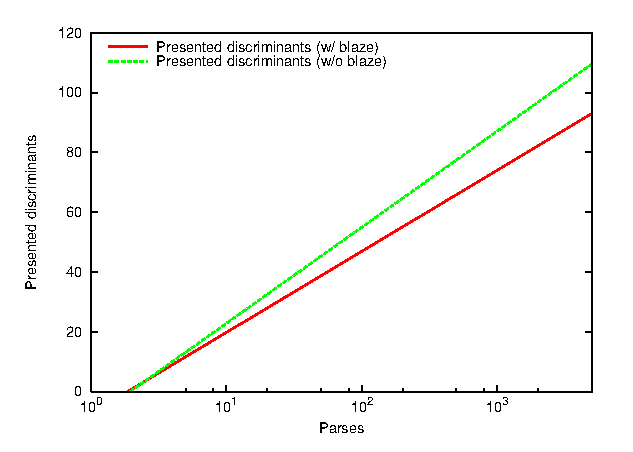
\includegraphics[width=0.7\textwidth]{include/parse-decision-presented.eps}
\begin{itemize}
\item Blazing POS tags reduced discriminants shown by 20\%
\end{itemize}


\myslide{Utterance Inter-annotator Agreement}
  \begin{tabular}{l|rrr|r}
      & $\alpha$ -- $\beta$  &  $\beta$ -- $\gamma$ & $\gamma$ -- $\alpha$ 
        & \textbf{Average}\\
      \hline
      Parse Agreement & 63.9\% &  68.2\% &  64.2\% &  65.4\% \\  
      Parse Disagreement & 17.5\% &  19.2\% &  17.9\% &  18.2\% \\  
      Reject Agreement &  4.8\%  &   3.0\%  &   4.1\%  &   4.0\% \\  
      Reject Disagreement & 13.7\%  &   9.5\%  &  13.8\%  &  12.4\% \\  
    \end{tabular}
\begin{itemize}
   \item  Total Agreement 69.4\%\
     \begin{itemize}
     \item \textit{cf} German NeGra corpus: 52\% (Newspaper text)
     \end{itemize}
   \item Average of 190 parses/sentence (10 words)
     % * (Parse agreement: $\kappa = .628$)
%   \item 現在の解析カバー率は84\%
   \end{itemize}

\myslide{Mutual Labeled Precision F-Score}

    \begin{tabular}{@{}c|rr|rr|rr|r@{}}
% Sherry = alpha
% Cognac = beta
% Port = gamma
\textbf{Test}           & \multicolumn{2}{|c|}{\textbf{$\alpha$ -- $\beta$}}
      & \multicolumn{2}{|c|}{\textbf{$\beta$ -- $\gamma$ }}
      & \multicolumn{2}{|c|}{\textbf{$\gamma$ -- $\alpha$}}
      & {\textbf{Average}}\\
\textbf{Set}           & \multicolumn{1}{|c}{\textbf{\#}}
      & \multicolumn{1}{c|}{\textbf{F}}
      & \multicolumn{1}{|c}{\textbf{\#}}
      & \multicolumn{1}{c|}{\textbf{F}}
      & \multicolumn{1}{|c}{\textbf{\#}}
      & \multicolumn{1}{c|}{\textbf{F}}
      & \multicolumn{1}{|c}{\textbf{F}}\\
      \hline
      \textbf{A} & 507 & 96.03 & 516 & 96.22 & 481 & 96.24 & 96.19\\
      \textbf{B} & 505 & 96.79 & 551 & 96.40 & 511 & 96.57 & 96.58\\
      \textbf{C} & 489 & 95.82 & 517 & 95.15 & 477 & 95.42 & 95.46\\
      \textbf{D} & 454 & 96.83 & 477 & 96.86 & 447 & 97.40 & 97.06\\
      \textbf{E} & 480 & 95.15 & 497 & 96.81 & 484 & 96.57 & 96.51\\
      \hline
       & 2435 & 96.32 & 2558 & 96.28  & 2400 & 96.47 & 96.36\\
    \end{tabular}

\myslide{Blazing Using POS scores}

 \begin{tabular}{ll}
  (verb-aux  & \iz{v-stem-lex} $-1.0$) \\
  (verb-main & \iz{aspect-stem-lex} $-1.0$)\\
  (noun      & \iz{verb-stem-lex} $-1.0$) \\
  (adnominal  & \iz{noun\_mod-lex-l} $0.9$ \\
                & \iz{det-lex} $0.9$)\\
  (conjunction& \iz{n\_conj-p-lex} $0.9$ \\
                 & \iz{v-coord-end-lex} $0.9$) \\
  (adjectival-noun & \iz{noun-lex} $-1.0$)
\end{tabular} 

\myslide{Number of Decisions}


  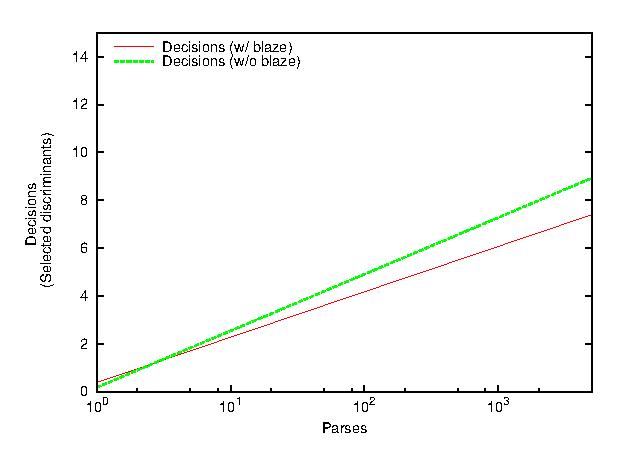
\includegraphics[width=0.7\textwidth]{include/parse-decision-selected.eps}

\begin{itemize}
\item Blazing  POS tags reduced decisions by 19.5\%
\end{itemize}


\myslide{Number of Decisions with Blazing}

  \begin{tabular}{crrrc}
\textbf{Test} & \multicolumn{3}{c}{\textbf{Annotator Decisions}}& \textbf{Blazed} \\
\textbf{Set} & $\alpha$ & $\beta$ & $\gamma$ & \textbf{Decisions}\\ \hline
%     Sherry         Cognac          Port          
\textbf{A} &   2,659         & 2,606         &  3,045          & 416\\
\textbf{B} &   2,848         & 2,939         &  \blu{2,253}  & 451\\
\textbf{C} &   \blu{1,930} & 2,487         &  2,882          & 468\\
\textbf{D} &   2,254         & \blu{2,157} &  2,347          & 397\\
\textbf{E} &   \blu{1,769} & \blu{2,278} &  \blu{1,811}  & 412\\ 
% A &   3745         & 2987         &  3838          & \\
% B &   2848         & 2939         &  \blu{2704}  & 451\\
% C &   \blu{2398} & 2487         &  2882          & 468\\
% D &   2254         & \blu{2554} &  2347          & 397\\
% E &   \blu{2181} & \blu{2690} &  \blu{2223}  & 412\\ 
  \end{tabular}


\myslide{Current Status}

\begin{itemize}
\item Finished treebanking\\[2ex]
%\item 対照コーパス:意味辞書Lexeedの語義文と例文(12.7万文)\\[2ex]
  \begin{tabular}{lrrr}
  Type  & Sentences & Words & Content Words\\ \hline
  Definition & 75,000 & 690,000 & 320,000 \\
  Example   & 46,000 & 500,000 & 220,000 \\
  \end{tabular}
\item But data not released by NTT, so I left them
\item Currently treebanking the Wordnet Definitions
%\item Exploit other lexicons ... 
%\item Use the grammar in other applications
%\item Treebank other genres
 \end{itemize}


\myslide{Conclusions}

\begin{itemize}
\item   5,000 sentences are annotated by three different annotators
\item  average inter-annotator agreement
  \begin{itemize}
  \item   65.4\% (sentence)
  \item  83.5\% using labeled precision
  \item 96.6\% on ambiguous annotated trees 
  \end{itemize}
\item blazing  POS tags reduced decisions by 19.5\%
\end{itemize}

\section{Lab 1}

\myslide{Non-exact matching}

\begin{itemize}
\item Often you will want to match not just a word or sequence of
  words but some kind of pattern
\item Various corpus interface tools make it easy to do this
\item A standard way is to match \txx{regular expressions}
\item A good text editor should allow regular expression matching
\\ e.g., EMACS, notepad++
\end{itemize}

\section{Regular Expressions}
\myslide{Regular Expressions}

\begin{itemize}
\item Regular expressions: a formal language for matching things.
\\[2ex]
  \begin{tabular}{ll}
    Symbol & Matches \\ \hline
    . & any single character\\
    {[ ]} & a single character that is contained within the brackets. \\
    & {[a-z]} specifies a range which matches any  letter from "a" to "z".\\
    {[\textasciicircum ~]} & 	a single character not in the brackets. \\
    \textasciicircum 	& the starting position within the string/line. \\
    \$ 	&  the ending position of the string/line. \\
    $*$ &	the preceding element zero or more times. \\
    ? &	 the preceding element zero or one time. \\
    + &	 the preceding element one or more times. \\
    $|$ &  either the expression before or after the operator. \\
    $\backslash$ & escapes the following character. \\
  \end{tabular}

\end{itemize}

\myslide{Regular Expression Examples}
\MyLogo{\url{http://www.regexplanet.com/simple/}}
\begin{itemize}
\item  \texttt{.at} matches any three-character string ending with "at", including "hat", "cat", and "bat".
\item \texttt{[hc]at} matches "hat" and "cat".
\item \texttt{[\textasciicircum{}b]at} matches all strings matched by \texttt{.at} except "bat".
\item \texttt{\textasciicircum{}[hc]at} matches "hat" and "cat", but only at the beginning of the string or line.
\item \texttt{[hc]at\$} matches "hat" and "cat", but only at the end of the string or line.
\item \texttt{$\backslash$[.$\backslash$]} matches any single character surrounded by "[" and "]" since the brackets are escaped, for example: "[a]" and "[b]".
\end{itemize}



\myslide{Wild Cards}
\MyLogo{}

\begin{itemize}
\item  a wildcard character  substitutes for any other character or characters in a string.
  \begin{itemize}
  \item \blu{Files and directories} (Unix, CP/M, DOS, Windows)
    \begin{description}
    \item[$*$] matches zero or more characters
    \item[?] matches one character
    \item[{[ ]}] matches a list or range of characters
    \end{description}
    \begin{itemize}
      \item E.g.:  Match any file that ends with the string ``.txt'' or ``.tex''.
\begin{verbatim}
ls *.txt *.tex
\end{verbatim}
     \end{itemize}
    \item \blu{Structured Query Language} (SQL)
    \begin{description}
    \item[\%]  matches zero or more characters
    \item[\_] matches a single character
    \end{description}
  \end{itemize}
\end{itemize}


\myslide{BYU Interface Specialties}
\MyLogo{\url{http://corpus.byu.edu/bnc/help/syntax_e.asp}}
\begin{small}
  \begin{tabular}{llll}
    Pattern & Explanation & Example & Matches \\ \hline
    word & One exact word & mysterious  & mysterious \\
    \texttt{[pos]} & Part of speech & \texttt{[vvg]} & going, using \\
    \texttt{[pos*]} & Part of speech & \texttt{[v*]} & find, does, keeping, started  \\
    \texttt{[lemma]} & Lemma & \texttt{[sing]} & sing, singing, sang \\
    \texttt{[=word]} & Synonyms & \texttt{[=strong]} & 	formidible, muscular, fervent \\
    word$|$wurd & Any of the words & stunning$|$gorgeous & stunning, gorgeous \\
    x?xx* & wildcards & on*ly & only, ontologically, on-the-fly, \\
    x?xx* & wildcards & s?ng & sing, sang, song \\
    -word & negation & \texttt{-[nn*]} & the, in, is \\
    \texttt{word.[pos]} & Word AND pos& can.\texttt{[v*]} &can, canning, canned (verbs)\\ 
& & can.\texttt{[n*]} & can, cans (nouns)\\
  \end{tabular}
\end{small}

%You can combine a \blu{word} restriction with a \blu{pos} restriction:


%%% Fixme double matches


\myslide{Acknowledgments}
\MyLogo{HG351 (2011)}

\begin{itemize}
\item Thanks to Na-Rae Han for 
  inspiration for some of the slides (from  \textit{LING 2050 Special Topics in Linguistics: Corpus linguistics}, U Penn).
\item Thanks to Sandra K\"{u}bler for some of the slides from her 
\textit{RoCoLi\footnote{Romania Computational Linguistics Summer School} Course: Computational Tools for Corpus Linguistics}
%\item Thanks to Mark Davies (BYU) for the exploration ideas.
\item Definitions from WordNet 3.0
\end{itemize}



%%
%% Future
%%


\end{document}

 
%%% Local Variables: 
%%% coding: utf-8
%%% mode: latex
%%% TeX-PDF-mode: t
%%% TeX-engine: xetex
%%% LaTeX-section-list:  (("myslide" 1))
%%% End: 